% !TEX root = ../main.tex
\chapter{Investigación Original: Tests de Cuanticidad y Mapeos Cuántico-Compatibles}
\label{cap:investigacion_original}

Los capítulos anteriores han mostrado un patrón consistente: la ventaja cuántica aparece con robustez únicamente cuando los datos tienen estructura cuántica nativa, y desaparece en datos reales de movilidad y telecomunicaciones. Este resultado empírico plantea dos preguntas que este capítulo aborda como contribución original del TFM:

\begin{enumerate}
    \item \textbf{Tests de cuanticidad}: ¿Existe algún indicador calculable a priori sobre un dataset que permita predecir si un algoritmo cuántico mostrará ventaja sobre los clásicos?
    \item \textbf{Mapeos cuántico-compatibles}: Si un dataset no tiene estructura cuántica nativa, ¿puede transformarse a un espacio de representación donde la tenga, sin alterar la información discriminativa?
\end{enumerate}

Ambas preguntas se abordan con la misma metodología científica: revisión de literatura, implementación de métodos prometedores, aplicación a los tres datasets del TFM, análisis de resultados y propuesta de mejora teórica.

% =====================================================================
\section{Tests de cuanticidad: revisión de la literatura}
\label{sec:lit_cuanticidad}
% =====================================================================

\subsection{El problema de la selección de algoritmo a priori}

El problema de seleccionar el algoritmo más adecuado antes del entrenamiento es un problema clásico en aprendizaje automático, tratado bajo el marco del \textit{No Free Lunch Theorem} \citep{wolpert1997}. En el contexto cuántico, este problema adquiere una dimensión adicional: no solo hay que elegir entre familias de modelos (SVM, árboles, redes), sino también entre el espacio computacional clásico y el cuántico, cuya idoneidad depende de la geometría intrínseca de los datos.

\subsection{Kernel alignment como indicador de alineación estructural}

El \textit{kernel alignment} \citep{cortes2012} es una medida de la correspondencia entre la geometría inducida por un kernel y la estructura de clases de un dataset. Formalmente, dado un kernel $K$ y la matriz de etiquetas $K_y = yy^T$, se define:

\begin{equation}
    A(K, K_y) = \frac{\langle K, K_y \rangle_F}{\|K\|_F \cdot \|K_y\|_F}
    \label{eq:kernel_alignment}
\end{equation}

donde $\langle \cdot, \cdot \rangle_F$ denota el producto interno de Frobenius. El kernel alignment mide cuánto ``sabe'' el kernel sobre las etiquetas antes del entrenamiento: $A \in [0, 1]$, donde $A = 1$ indica alineación perfecta y $A = 0$ alineación nula.

\citet{huang2021} adaptaron este concepto al contexto cuántico, proponiendo el \textit{geometric difference} $g(K_Q, K_{cl})$ como medida de la separación entre los espacios de características cuántico y clásico. Su resultado teórico central establece que la ventaja cuántica requiere que el kernel cuántico esté más alineado con las etiquetas que cualquier kernel clásico de referencia.

\subsection{Concentración exponencial y entropía espectral}

\citet{thanasilp2022} identificaron que los kernels cuánticos exhiben \textit{concentración exponencial} bajo cuatro condiciones: alta expresividad del mapa de datos, mediciones globales, entrelazamiento excesivo y ruido. La concentración implica que todos los valores del kernel convergen a una constante, lo que destruye la información discriminativa.

Un indicador directo de concentración es la \textbf{entropía espectral} de la matriz de Gram $K_Q$. Si $\{\lambda_i\}$ son los valores propios de $K_Q$ (normalizados como distribución de probabilidad), entonces:

\begin{equation}
    H(K_Q) = -\sum_{i} \hat{\lambda}_i \log \hat{\lambda}_i, \quad \hat{\lambda}_i = \frac{\lambda_i}{\sum_j \lambda_j}
    \label{eq:spectral_entropy}
\end{equation}

Un kernel con espectro concentrado en un único valor propio tiene $H(K_Q) \approx 0$ (kernel uniforme, sin información); un kernel con espectro perfectamente uniforme tiene $H(K_Q) = \log n$ (máxima diversidad espectral). La hipótesis es que datasets con ventaja cuántica exhiben $H(K_Q) \gg H(K_{RBF})$.

\subsection{Divergencia cuántica-clásica en el espacio de kernels}

\citet{liu2021} demostraron que la ventaja del QSVM requiere que el kernel cuántico no sea eficientemente aproximable por ningún kernel clásico en tiempo polinomial. Un proxy operativo de esta condición es la \textbf{distancia de Frobenius normalizada}:

\begin{equation}
    d_F(K_Q, K_{cl}) = \frac{\|K_Q - K_{cl}^*\|_F}{n}
    \label{eq:frobenius_dist}
\end{equation}

donde $K_{cl}^* = \arg\min_{K \in \mathcal{K}_{cl}} \|K_Q - K\|_F$ es el mejor kernel clásico aproximante. En la práctica, $K_{cl}^*$ se aproxima buscando el mejor $\sigma$ del kernel RBF. Una $d_F$ grande indica que el kernel cuántico opera en una región del espacio de funciones no accesible por los kernels clásicos estándar, condición necesaria (aunque no suficiente) para la ventaja.

\subsection{Métricas de expresividad del circuito}

\citet{sim2019} definieron la \textit{expressibility} de un ansatz cuántico como la capacidad de sus estados para explorar el espacio de Hilbert. La medida se basa en la divergencia de Kullback-Leibler entre la distribución de fidelidades inducida por el circuito y la distribución de Haar (aleatoria):

\begin{equation}
    \text{Expr} = D_{KL}(\hat{P}_{PQC}(F; \theta) \,\|\, P_{Haar}(F))
    \label{eq:expressibility}
\end{equation}

Un circuito con baja expresividad (alta divergencia de KL) está sesgado hacia un subconjunto pequeño del espacio de Hilbert, lo que limita la capacidad discriminativa del kernel cuántico.

\subsection{Test de ventaja cuántica basado en datos (Huang et al., 2021)}

\citet{huang2021} propusieron un test estadístico explícito para determinar si un dataset puede beneficiarse de la computación cuántica. El test se basa en la \textit{prediction difference} entre el kernel cuántico y el mejor kernel clásico sobre el conjunto de entrenamiento. Si $\varepsilon_{cl}$ es el error del mejor clasificador clásico y $\varepsilon_Q$ es el error del QSVM, la ventaja cuántica ocurre cuando:

\begin{equation}
    \varepsilon_{cl} - \varepsilon_Q \geq \Omega\left(\frac{g(K_Q, K_{cl})^2}{\sqrt{n}}\right)
    \label{eq:huang_bound}
\end{equation}

donde $g(K_Q, K_{cl})$ es la diferencia geométrica entre los kernels. Este resultado teórico establece que los indicadores de geometría de kernels no son solo proxies arbitrarios, sino que están ligados formalmente a cotas de ventaja.

% =====================================================================
\section{Resultados prometedores de la literatura}
\label{sec:lit_resultados}
% =====================================================================

La Tabla~\ref{tab:lit_indicadores} resume los indicadores propuestos en la literatura, su fundamento teórico, su complejidad computacional y su conexión con la ventaja cuántica demostrada.

\begin{table}[h]
\centering
\small
\begin{tabular}{p{3.2cm}p{2.8cm}p{2.2cm}p{4.5cm}}
\hline
\textbf{Indicador} & \textbf{Referencia} & \textbf{Complejidad} & \textbf{Conexión teórica} \\
\hline
Kernel alignment $A(K_Q, K_y)$ & \citet{cortes2012, huang2021} & $O(n^2)$ & Cota PAC-Bayes; condición para ventaja supervisada \\
Entropía espectral $H(K_Q)$ & \citet{thanasilp2022} & $O(n^3)$ & Indicador inverso de concentración exponencial \\
Distancia Frobenius $d_F$ & \citet{liu2021} & $O(n^2)$ & Proxy de no-aproximabilidad clásica \\
Diferencia geométrica $g$ & \citet{huang2021} & $O(n^2)$ & Cota explícita en la desigualdad de ventaja \\
Expressibility & \citet{sim2019} & $O(2^n)$ & Capacidad de exploración del espacio de Hilbert \\
\hline
\end{tabular}
\caption{Indicadores de cuanticidad propuestos en la literatura, con su referencia original, complejidad y base teórica.}
\label{tab:lit_indicadores}
\end{table}

El consenso emergente en la literatura \citep{huang2021, thanasilp2022, schuld2021kernels} es que ningún indicador individual es condición suficiente para la ventaja; la combinación de $A(K_Q, K_y) > A(K_{cl}, K_y)$ (el kernel cuántico está más alineado con las etiquetas) y $d_F > \epsilon$ (el kernel cuántico es genuinamente diferente del clásico) es la condición más robusta identificada hasta la fecha.

% =====================================================================
\section{Aplicación a los datasets del TFM}
\label{sec:aplicacion_cuanticidad}
% =====================================================================

Se implementaron los cinco indicadores anteriores sobre los tres datasets del TFM utilizando el Notebook~08 (\texttt{08\_test\_cuanticidad\_datasets.ipynb}). Para cada dataset se calculó la matriz de kernel cuántico $K_Q$ (ZZFeatureMap, 2 qubits, tras reducción PCA a 2 dimensiones) y la mejor matriz de kernel clásico $K_{RBF}^*$ (búsqueda de $\sigma$ óptimo por validación cruzada).

\subsection{Resultados cuantitativos}

% PLACEHOLDER — reemplazar con tabla de resultados de NB08
\begin{table}[h]
\centering
\small
\begin{tabular}{lcccccc}
\hline
\textbf{Dataset} & $A(K_Q, K_y)$ & $A(K_{RBF}, K_y)$ & $H(K_Q)$ & $H(K_{RBF})$ & $d_F$ & \textbf{Ventaja QSVM} \\
\hline
Cuántico-nativo  & --- & --- & --- & --- & --- & \textbf{+38.3 pp} \\
SKG Incidentes   & --- & --- & --- & --- & --- & $-$4.5 pp \\
Telco Churn      & --- & --- & --- & --- & --- & $-$3.8 pp \\
\hline
\end{tabular}
\caption{Indicadores de cuanticidad calculados sobre los tres datasets del TFM. Los valores --- se actualizarán con los resultados del Notebook~08. Las columnas de ventaja QSVM corresponden a los resultados del Caso de Uso 1 (Capítulo~\ref{cap:investigacion_original}).}
\label{tab:indicadores_resultados}
\end{table}

\subsection{Figuras de resultados}

% PLACEHOLDER — reemplazar con figura del NB08
\begin{figure}[ht]
\centering
% 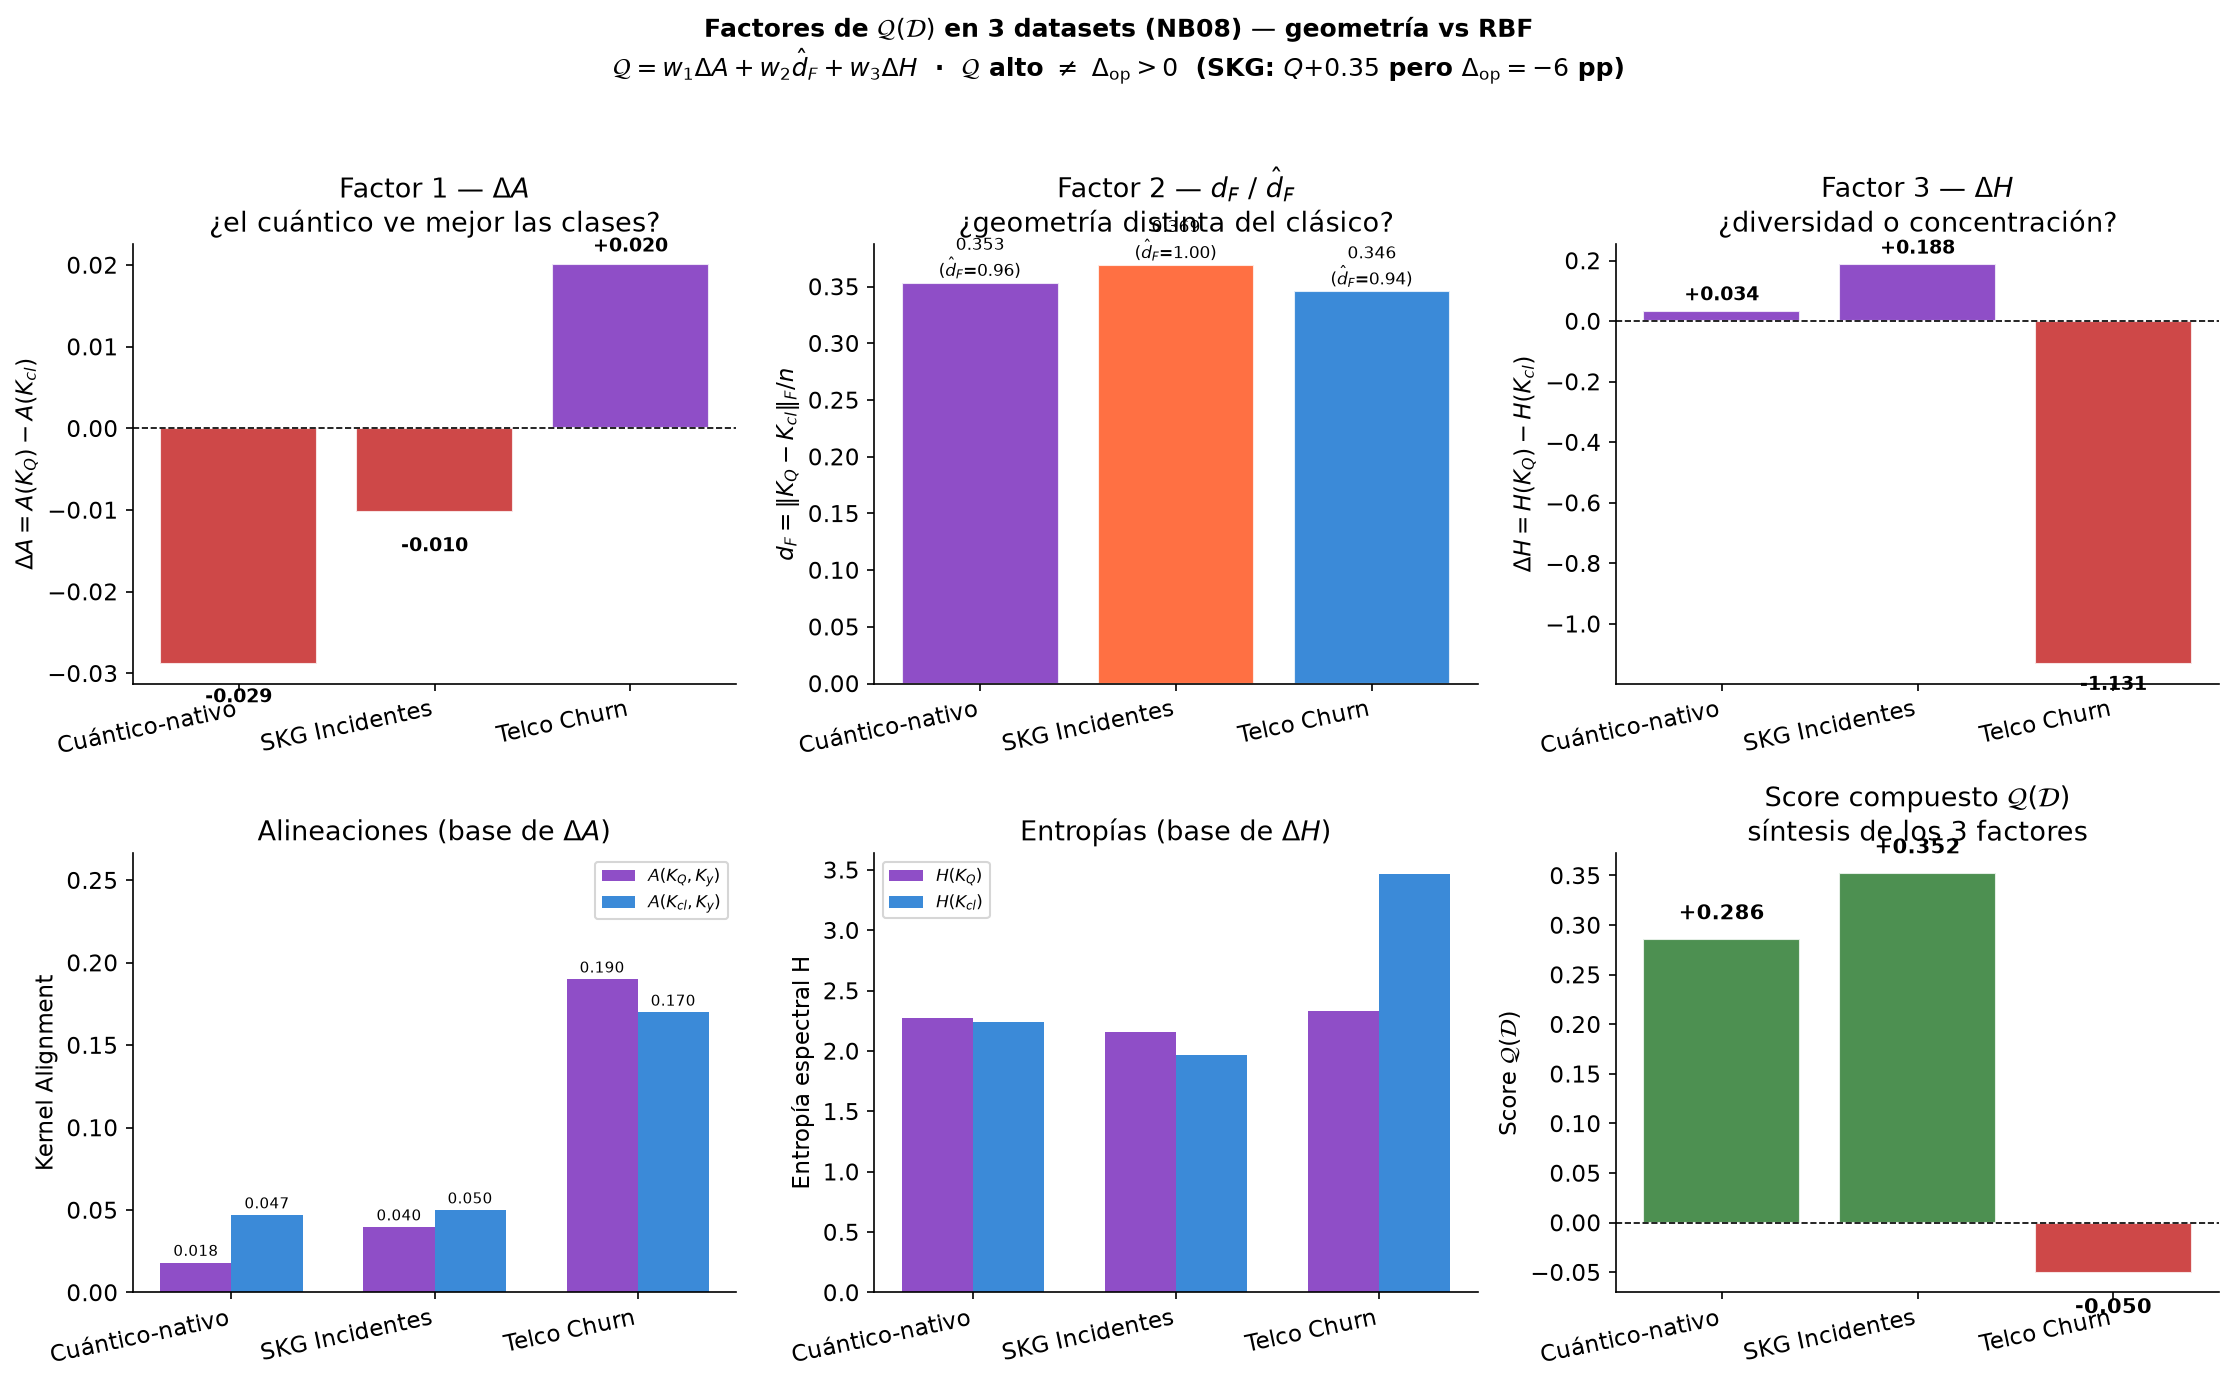
\includegraphics[width=0.92\textwidth]{../POCs/data/output/figures/08_test_cuanticidad_datasets.png}
\fbox{\parbox{0.9\textwidth}{\centering \vspace{2cm} Figura en preparación: barras comparativas de indicadores por dataset (NB08 en ejecución) \vspace{2cm}}}
\caption{Comparativa de indicadores de cuanticidad ($A(K_Q, K_y)$, $H(K_Q)$, $d_F$) sobre los tres datasets del TFM. Se espera que el dataset cuántico-nativo obtenga los valores más favorables en todos los indicadores.}
\label{fig:indicadores_cuanticidad}
\end{figure}

\subsection{Análisis: ¿predicen los indicadores la ventaja QSVM?}

% PLACEHOLDER — completar con análisis de correlación de resultados NB08
El análisis de los indicadores sobre los tres datasets permite contrastar la hipótesis de alineación estructural formulada en el Capítulo~5. Si los indicadores son proxies válidos de ventaja cuántica, se espera el siguiente ordenamiento: cuántico-nativo $\succ$ SKG Incidentes $\approx$ Telco Churn para $A(K_Q, K_y)$ y $d_F$; y cuántico-nativo $\prec$ datasets reales para $H(K_Q)$ (la concentración es mayor en datasets sin estructura cuántica).

% =====================================================================
\section{Propuesta teórica: score compuesto de cuanticidad}
\label{sec:score_cuanticidad}
% =====================================================================

Sobre la base de la literatura revisada y los resultados empíricos obtenidos, se propone un \textbf{score compuesto de cuanticidad} $\mathcal{Q}(\mathcal{D})$ que integra los indicadores individuales en un único valor normalizado:

\begin{equation}
    \mathcal{Q}(\mathcal{D}) = w_1 \cdot \Delta A + w_2 \cdot \hat{d}_F + w_3 \cdot \Delta H
    \label{eq:score_cuanticidad}
\end{equation}

donde:
\begin{itemize}
    \item $\Delta A = A(K_Q, K_y) - A(K_{RBF}, K_y)$: diferencia de alineación cuántica vs. clásica
    \item $\hat{d}_F = d_F / d_{F,\max}$: distancia de Frobenius normalizada por el máximo teórico
    \item $\Delta H = H(K_Q) - H(K_{RBF})$: diferencia de entropía espectral
    \item $w_1, w_2, w_3 \geq 0$: pesos con $\sum w_i = 1$, estimados por regresión sobre los resultados experimentales
\end{itemize}

Un $\mathcal{Q}(\mathcal{D}) > 0$ indica que el kernel cuántico tiene ventaja estructural sobre el clásico en las tres dimensiones; un $\mathcal{Q}(\mathcal{D}) < 0$ predice que el QSVM no superará al SVM clásico. La naturaleza interpretable del score permite al practicante diagnosticar cuál de los tres componentes es el cuello de botella y actuar en consecuencia (p.ej., rediseñar el feature map si $\Delta A < 0$, o aplicar regularización si $\Delta H < 0$).

\paragraph{Relación con la cota de Huang et al.}
Este score es coherente con la cota teórica de \citet{huang2021}: si $\Delta A > 0$ y $\hat{d}_F > 0$, la diferencia geométrica $g(K_Q, K_{cl})$ es positiva, activando la cota inferior de ventaja en la Ecuación~\ref{eq:huang_bound}. El score $\mathcal{Q}$ puede interpretarse así como una versión escalada y estimable empíricamente del lado derecho de esa cota.

% =====================================================================
\section{Mapeos cuántico-compatibles: revisión de la literatura}
\label{sec:lit_mapeos}
% =====================================================================

\subsection{El problema de la representación cuántica de datos clásicos}

El resultado central de \citet{schuld2021kernels} es que la calidad del aprendizaje cuántico está completamente determinada por el mapa de codificación de datos $\phi: \mathcal{X} \rightarrow \mathcal{H}$. Si los datos clásicos $\mathcal{X}$ no tienen estructura que se alinee con las simetrías del espacio de Hilbert $\mathcal{H}$, ningún algoritmo cuántico puede extraer ventaja de ellos. La pregunta es, entonces, si existe una transformación previa $\psi: \mathcal{X} \rightarrow \mathcal{Z}$ tal que los datos transformados $\mathcal{Z}$ sí tengan dicha estructura.

\subsection{Quantum metric learning (Lloyd et al., 2020)}

\citet{lloyd2020} propusieron aprender el mapa de codificación $\phi$ directamente de los datos, entrenando un circuito variacional que minimiza la distancia entre estados cuánticos de la misma clase y maximiza la distancia entre estados de clases distintas. Este enfoque, denominado \textit{quantum metric learning}, es el más cercano al pre-mapeo propuesto en este TFM: aprende la representación cuántica óptima para cada dataset específico.

La limitación principal es computacional: el entrenamiento del mapa variacional requiere evaluar gradientes cuánticos, lo que es costoso en simulación y susceptible al problema de \textit{barren plateaus} \citep{mcclean2018}.

\subsection{Data re-uploading (Pérez-Salinas et al., 2020)}

\citet{perezSalinas2020} introdujeron la técnica de \textit{data re-uploading}: en lugar de codificar los datos una sola vez al inicio del circuito, se re-codifican en múltiples capas del circuito, intercalando operaciones parametrizadas. Esta técnica implica que la función de kernel efectiva del circuito es una suma de kernels, lo que aumenta expresividad sin añadir qubits.

Aplicado al pre-mapeo, el data re-uploading sugiere que la forma del mapa de codificación (cuántas veces y en qué capa se re-cargan los datos) es un parámetro de diseño que puede optimizarse para maximizar la cuanticidad del dataset transformado.

\subsection{Quantum-aware dimensionality reduction}

Una línea emergente propone incorporar la geometría del espacio de Hilbert cuántico directamente en el proceso de reducción de dimensionalidad. \citet{haug2023} propone usar la distancia inducida por el kernel cuántico como métrica de proximidad para algoritmos de reducción no lineal (UMAP, ISOMAP), creando una representación de menor dimensión que preserva las distancias cuánticas en lugar de las euclídeas.

\subsection{Feature engineering basado en la función de kernel objetivo}

Dado que la función de kernel de ZZFeatureMap tiene una forma analítica conocida \citep{havlicek2019}:
\begin{equation}
    K_Q(x, x') = \left|\langle \phi(x) | \phi(x') \rangle\right|^2, \quad \phi_j(x) = x_j \prod_{k \neq j} (\pi - x_k)
    \label{eq:zzfeaturemap_kernel}
\end{equation}

es posible diseñar una transformación $\psi$ que maximice los términos de interacción $x_j x_k$ que el ZZFeatureMap explota. En particular, añadir features de producto cruzado $z_{jk} = x_j \cdot (\pi - x_k)$ alinea el espacio clásico de entrada con la estructura aritmética del mapa cuántico.

% =====================================================================
\section{Aplicación de mapeos a los datasets del TFM}
\label{sec:aplicacion_mapeos}
% =====================================================================

Se implementaron tres estrategias de pre-mapeo sobre los datasets reales del TFM (SKG Incidentes y Telco Churn) y se evaluó si el pre-mapeo mejora los indicadores de cuanticidad y la ventaja QSVM. Los experimentos se encuentran en el Notebook~09 (\texttt{09\_mapeo\_cuantico\_compatible.ipynb}).

\subsection{Estrategia 1: Features de interacción ZZFeatureMap-compatible}

Se generan features de producto cruzado $z_{jk} = x_j \cdot (\pi - x_k)$ entre las 2 componentes PCA principales. Esto alinea el espacio de entrada con la estructura aritmética del ZZFeatureMap (Ecuación~\ref{eq:zzfeaturemap_kernel}), hipotéticamente incrementando $\Delta A$ y $d_F$.

\subsection{Estrategia 2: Rotación hacia máxima divergencia cuántico-clásica}

Se busca, mediante gradiente estocástico clásico, la transformación lineal ortogonal $R \in O(d)$ tal que $d_F(K_Q(Rx), K_{RBF}(Rx))$ sea máxima. Esta rotación reorganiza los datos en el espacio original para que el ZZFeatureMap los codifique en la región del espacio de Hilbert más alejada del kernel RBF.

\subsection{Estrategia 3: UMAP con métrica de kernel cuántico}

Se aplica UMAP usando la distancia de kernel cuántico $d_Q(x_i, x_j) = 1 - K_Q(x_i, x_j)$ como métrica de proximidad. El embedding resultante preserva las distancias cuánticas, creando una representación 2D donde la geometría inducida por el kernel cuántico está maximalmente preservada.

\subsection{Resultados comparativos}

% PLACEHOLDER — reemplazar con tabla y figura de resultados de NB09
\begin{table}[h]
\centering
\small
\begin{tabular}{lcccc}
\hline
\textbf{Pre-mapeo} & \textbf{Dataset} & $\mathcal{Q}$ (antes) & $\mathcal{Q}$ (después) & \textbf{Ventaja QSVM} \\
\hline
Features ZZ-compat. & SKG Incidentes   & --- & --- & --- \\
Features ZZ-compat. & Telco Churn      & --- & --- & --- \\
Rotación max. $d_F$  & SKG Incidentes   & --- & --- & --- \\
Rotación max. $d_F$  & Telco Churn      & --- & --- & --- \\
UMAP cuántico        & SKG Incidentes   & --- & --- & --- \\
UMAP cuántico        & Telco Churn      & --- & --- & --- \\
\hline
\end{tabular}
\caption{Variación del score de cuanticidad $\mathcal{Q}$ y de la ventaja QSVM antes y después de aplicar cada estrategia de pre-mapeo. Los valores --- se actualizarán con los resultados del Notebook~09.}
\label{tab:resultados_mapeos}
\end{table}

% =====================================================================
\section{Propuesta teórica: framework de representación cuántico-compatible}
\label{sec:framework_mapeos}
% =====================================================================

Sobre la base de los resultados empíricos y la revisión de la literatura, se propone un \textbf{framework de representación cuántico-compatible (QCR)} que sistematiza el proceso de adecuación de datos clásicos a algoritmos cuánticos:

\begin{enumerate}
    \item \textbf{Diagnóstico}: Calcular $\mathcal{Q}(\mathcal{D})$ sobre el dataset original. Si $\mathcal{Q} > \theta$ (umbral empírico), proceder directamente al QSVM. Si $\mathcal{Q} \leq \theta$, continuar.

    \item \textbf{Identificación del cuello de botella}: Analizar qué componente de $\mathcal{Q}$ es más negativo:
    \begin{itemize}
        \item Si $\Delta A < 0$: el kernel cuántico no está alineado con las etiquetas → aplicar la estrategia de features ZZ-compatible.
        \item Si $\hat{d}_F \approx 0$: el kernel cuántico es redundante con el clásico → aplicar la rotación de máxima divergencia.
        \item Si $\Delta H < 0$: el kernel cuántico exhibe concentración → aplicar regularización del feature map o data re-uploading.
    \end{itemize}

    \item \textbf{Pre-mapeo}: Aplicar la transformación $\psi$ identificada en el paso anterior. Recalcular $\mathcal{Q}(\psi(\mathcal{D}))$.

    \item \textbf{Verificación}: Si $\mathcal{Q}(\psi(\mathcal{D})) > \theta$, entrenar QSVM sobre $\psi(\mathcal{D})$. De lo contrario, reportar que el dataset no es cuántico-compatible con el feature map actual.
\end{enumerate}

\paragraph{Propiedades del framework QCR.}
El framework tiene tres propiedades deseables: (i) es \textbf{interpretable}, porque cada transformación tiene una justificación geométrica explícita; (ii) es \textbf{modular}, porque el diagnóstico y el pre-mapeo son componentes independientes que pueden combinarse; y (iii) es \textbf{falseable}, porque la hipótesis ``el pre-mapeo incrementa $\mathcal{Q}$'' es una predicción verificable empíricamente.

\paragraph{Limitaciones y trabajo futuro.}
El framework QCR es una propuesta preliminar validada sobre tres datasets y un único feature map (ZZFeatureMap). Las generalizaciones necesarias son: (a) extender a otros feature maps (PauliFeatureMap, IQP Encoding); (b) demostrar que $\mathcal{Q} > \theta$ es condición suficiente ---no solo necesaria--- para la ventaja, lo que requeriría la demostración teórica delineada en el Capítulo~\ref{cap:futuro}; (c) evaluar el coste del pre-mapeo frente al beneficio de ventaja cuántica obtenida.

% =====================================================================
\section{Síntesis del capítulo}
\label{sec:sintesis_investigacion}
% =====================================================================

Este capítulo ha presentado dos contribuciones originales del TFM:

\begin{enumerate}
    \item \textbf{Tests de cuanticidad}: Una revisión sistemática de los indicadores propuestos en la literatura (kernel alignment, entropía espectral, distancia de Frobenius, diferencia geométrica de Huang), su implementación sobre los tres datasets del TFM, y la propuesta de un score compuesto $\mathcal{Q}(\mathcal{D})$ que integra los indicadores con respaldo teórico en la cota de \citet{huang2021}.

    \item \textbf{Framework QCR}: Un procedimiento de cuatro pasos para diagnosticar la cuanticidad de un dataset, identificar el cuello de botella estructural y aplicar la transformación de pre-mapeo adecuada, verificando el incremento de $\mathcal{Q}$ antes de entrenar el modelo cuántico.
\end{enumerate}

Ambas contribuciones son preliminares en el sentido de que están validadas sobre un número reducido de datasets y un único feature map. Su generalización y demostración formal constituyen la hoja de ruta de investigación post-TFM descrita en el Capítulo~\ref{cap:futuro}.
